\section{Phase 1: Analyse}

\subsection{Beschreibung möglicher Anwendungen aus Business-Sicht}
\label{ref:businessSicht}

Um den längerfristigen Erfolg eines Unternehmen zu gewährleisten, ist es notwendig Kennzahl und Faktoren für dieses zu definieren. 
Aus den gegebenen Zahlen lassen sich verschiedene Perspektiven ableiten. 
Die somit definierten Perspektiven sollten finanzielle Aspekte berücksichtigen, das Kaufverhalten des Kunden veranschaulichen und die Entwicklung des Unternehmens allgemein beschreiben.\\
Im folgenden werden die einzelnen Perspektiven: Finanzperspektive, Kundenperspektive und Entwicklungsperspektive vorgestellt.

\begin{table}[htbp]
\textbf{Finanzperspektive}
\begin{center}
  \begin{tabular}{ | l | r | }
    \hline
    \textbf{Ziel oder Fragestellung} & \textbf{Kennzahlen} \\ \hline
	Wieviel kauft das Bundesland? & Vergleich Verkaufsanzahl zu Einwohnerzahl\\     
     Kaufkraft der Bundesländer & (Quantität, zeitlich, ortsbezogen) \\  im Verhältnis zur Einwohnerzahl &  \\ \hline
    Wie wirkt sich die Farbe eines Artikels & Artikeleigenschaft (Farbe),  \\ auf den Preis und den & Preis und Verkaufsanzahl \\   verkauften Einheiten aus? &  \\ \hline
    Wie hoch ist die Marge einer Artikelgruppe? & Marktwert der Rohstoffe und Preis \\Preise von Artikelgruppen im zshg. & von ausgewählten Artikelgruppen  \\  mit dem Markwert von Rohstoffen & (z.B.: Shirt)\\ \hline
  \end{tabular}
\end{center}
\caption{Finanzperspektive}
\label{table:tableFinanz}
\end{table}

\begin{table}[htbp]
\textbf{Kundenperspektive}
\begin{center}
  \begin{tabular}{ | l | r | }
    \hline
    \textbf{Ziel oder Fragestellung} & \textbf{Kennzahlen} \\ \hline
	Werden die Rechnungen von & Eigenschaften von \\ einer anderen Person gezahlt?   & Kunde mit Bestellung \\  Welcher Altersgruppe gehört der zahlende an?  & und zahlenden Kunden \\ Analyse des Kaufverhaltens & 
    \\ \hline
    Zshg. von Körpergröße mit & Eigenschaften Artikel (Größe), \\ online/offline Einkäufen & Eigenschaften Bestellung (online), \\ und Retourenanzahl & und Anzahl der Retouren \\ \hline
  \end{tabular}
\end{center}
\caption{Kundenperspektive}
\label{table:tableKunde}
\end{table}

\pagebreak 

\begin{table}[htbp]
\textbf{Entwicklungsperspektive}
\begin{center}
  \begin{tabular}{ | l | r | }
    \hline
    \textbf{Ziel oder Fragestellung} & \textbf{Kennzahlen} \\ \hline
    Welche Artikelgruppe (z.B.: Shirt) & Verkauf von ausgewählten \\ wird wann in welchen Bundesland &   Artikelgruppen pro Land und \\ verkauft und wie teuer wäre die Herstellung? & Zeit mit Rohstoffpreis \\ \hline
    Wie zahlen die Generationen? & Umsatz nach Alter pro Jahr \\ \hline
    Wer kauft online o. offline, & Eigenschaften Bestellung, \\ nach Altersgruppe und Bundesland & Ort und Alter des Kunden \\ \hline 
  \end{tabular}
\end{center}
\caption{Entwicklungsperspektive}
\label{table:tableEntwicklung}
\end{table}
\vspace{1.0cm}
\textbf{Besonderheiten der Zielstellungen}

Die gestellten Ziele und Fragestellungen beziehen sich nicht auf übliche Auswertungen, wie etwa die Lebendsdauer eines Kunden oder Warenkorbanalysen.
Die gegebenen Kennzahlen wurden so gewählt, dass möglichst interessante Fragestellungen trotz des Verzichts behandelter Abfragen der Seminarserien entstanden.
Für die Umsetzung dieser Analysen muss neben der Arbeit auf den gegebenen Daten ein Mehraufwand getätigt werden.
Zum einen müssen für die Auswertungen externe Quellen verwendet werden, wie etwa für die Rohstoffe oder die Zuordnung der Postleitzahl zu den Bundesländern. 
Zum anderen müssen selbst definierte Gruppierungen gebildet werden, wie etwa die Artikelgruppe ''Shirts''.

\pagebreak
\subsection{Konzeptuelle Modellierung}
\label{ref:modellierung}
\subsection*{Cube Bestellungen}
\begin{figure}[htbp] 
  \centering
    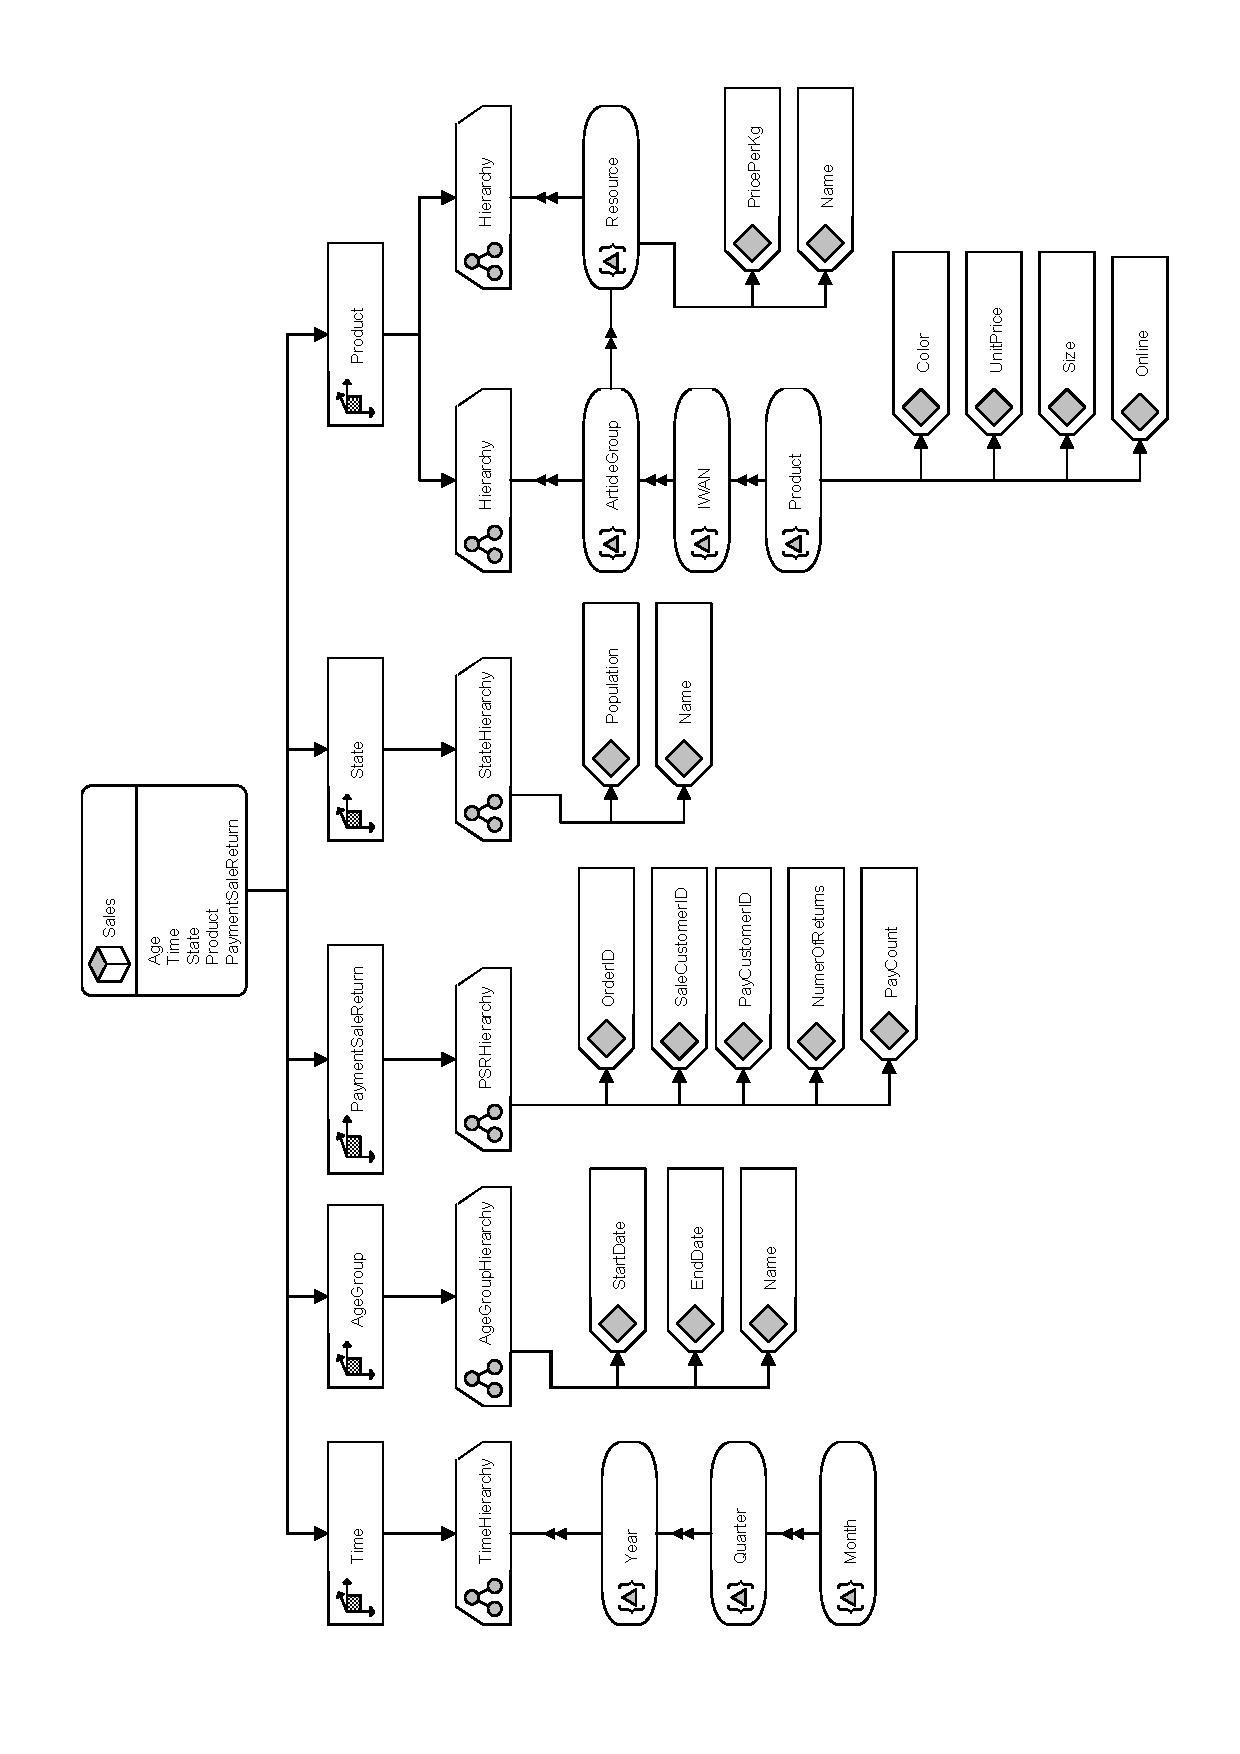
\includepdf[angle=-90,scale=0.9,offset=-0.2cm 3.5cm]{phase1/cube.pdf}
    \caption*{}
\end{figure}

\vspace{11cm}

Der dargestellte Cube soll für alle angeforderten Auswertungen verwendet werden. 
Neben den Standard-Hierarchien wie Zeit, Altersgruppe oder Ort (\texttt{State}) gibt es auch die Produktdimension und die Dimension der abgeschlossenen Bestellungen (\texttt{PaymentSaleReturn}). 
Produktspezifische Auswertungen wie die Eigenschaften eines Artikels als auch die Eigenschaften von Artikelgruppen, wie die verbrauchten Ressourcen, können mit der Produktdimension getätigt werden. 
Alle zahlungstechnischen Details einer Bestellung oder Retoure (z.B. Wer zahlt die Rechnung?), werden in der Dimension der \texttt{PaymentSaleReturn}-Dimension zur Verfügung gestellt.

\subsection{Datenverarbeitungsanforderungen}
\label{ref:businessSicht}
\subsection*{Finanzperspektive}

Im finanziellen Sektor stellen wir uns die Frage, wie die Kaufkraft in Abhängigkeit von der Einwohnerzahl (erhoben 2015) auf alle Bundesländer verteilt ist. Diese Auswertung kann einmal jährlich vorgenommen werden, um eine Tendenz zu beschreiben. Einwohnerzahlen werden jährlich erhoben, folgen aber einer berechenbaren Wachstumsrate, so dass man mit einem festen Wert rechnen kann. Zugleich kann man auch einen monatliche Report ausgeben, doch dieser würde keinen Trend anzeigen.
 
Bei der Auswahl eines Produktes fällt das Aussehen zu 90\% ins Gewicht. Es ist zu prüfen, welches Produkt in welcher Farbe die höchsten Absätze generiert. Bei neuen Produkten kann diese Analyse schon wöchentlich geschehen, damit nicht rentable Produktfarben ausgeschlossen werden können. Diese Aussage hat allerdings keinen Einfluss auf die Qualität eines Produktes oder ob der Erfolg davon abhängig ist. Ein schlechtes Produkt ist auch in einer schönen Farbe schlecht. Man kann nur eine Aussage über die Vorliebe einer Farbe treffen und kann so eine Vorausplanung machen, wie oft das Produkt in der Farbe verkauft wird.
 
Das dritte Ziel der Finanzanalyse soll eine grobe Übersicht zwischen dem Preis des Rohstoffes und dem Verkaufspreis sein. Die Produkte werden in Artikelgruppen eingeordnet und diesen dann Rohstoffen. Hier werden hauptsächlich Textilien verkauft, daher wurden Rohstoffpreise für Baumwolle, Seide, Leder und Polyester aus dem Jahr 2012 ermittelt. Pro Artikelgruppe wird auch ein durchschnittliches Gewicht berechnet und so der Herstellungspreis bestimmt. Diese Aussage ist nicht sehr genau, da Kosten für Verwaltung, Transport usw. fehlen. 
 
\subsection*{Kundenperspektive}
 
Unser erstes Ziel ist es, in Erfahrung zu bringen wer die Rechnung der Bestellung bezahlt. Hier können Kunden gefiltert werden, die sich ihre Bestellungen bezahlen lassen. Die Schlussfolgerung daraus ist weit interpretierbar. Zum Beispiel kann angenommen werden, dass es sich um ein Geschenk handelt oder ob die Großeltern/Eltern häufig die Rechnungen begleichen. Hier kann nur mit dem Alter eine Aussage getroffen werden, da die Namen anonymisiert wurden. Wird die Rechnung z.B. von jemanden bezahlt der 20 Jahre älter ist, so kann es sich um ein Elternteil handeln. Allerdings ist auch hier der Report nicht sehr aussagekräftig, da es sich hier auch um Geschwister, Verwandte oder Freunde handeln kann. In Kombination mit dem Nachnamen und der Stadt kann diese Aussage allerdings genauer werden. 
Gleichzeitig kann ermittelt werden, welche Altersgruppe in dieser Filiale einkauft und welchen Betrag sie monatlich/jährlich da lässt. Diese Angaben sind sehr genau, da Alter und Betrag eines Kunden erfasst werden. Diese Analyse monatlich auszuführen ist überflüssig, da eine gute Aussage erst auf lange Sicht möglich ist. 
 
Unser drittes Ziel ist es, in Erfahrung zu bringen, ob Menschen mit einem großen Körperindex eher Online-Einkäufe tätigen oder ob es keinen Unterschied zu dem lokalen Einkauf gibt. Zugleich kann in Erfahrung gebracht werden, ob sich der Ausbau eines Onlinehandels lohnt. Hier gibt es genaue Zahlen, welche Produkte online gekauft wurden, in welcher Größe und auch wie oft. Es kann also eine zuverlässige Aussage getroffen werden. Doch man muss beachten, dass man mit der Körpergröße nicht gleich auf den Körperumfang schließen kann. Die Retourenanzahl ist zudem ein Faktor, um zu ermitteln, welcher Kunde mehr Kosten als Nutzen verursacht. Auch hier können genaue Zahlen gemacht werden. Dieser Report sollte monatlich ausgewertet werden.
 
 
\subsection*{Entwicklungsperspektive}
 
Unser erstes Ziel kann mit der Finanzanalyse verbunden werden und kann darauf Bezug nehmen.
 
Ein interessanter Fakt ist der Einkauf der verschiedenen Altersgruppen. Zahlen Ältere eher Bar und die Jungen eher mit Karte? Diese Daten sind sehr genau in der Datenbank hinterlegt und können auch wöchentlich ausgewertet werden. Je nach Aktualität der Datenbank können auch Echtzeitanalysen erhoben werden. Hier kann nebenbei untersucht werden, ob z.B. die Terminals einer Filiale ausgefallen sind, weil auf einmal nur noch Bar bezahlt wird. Ursachen können fehlerhafte Geräte oder Einbruch des Banksystem sein. Um eine genau Aussage zu treffen, müssen die Daten in Echtzeit ausgewertet werden und mögliche andere Fehlerquellen (wie z.B. Ausfall der Internetverbindung) berücksichtigt werden.

\pagebreak
